\documentclass[conference]{IEEEtran}
\IEEEoverridecommandlockouts
% The preceding line is only needed to identify funding in the first footnote. If that is unneeded, please comment it out.
\usepackage{cite}
\usepackage{hyperref}
\usepackage{amsmath,amssymb,amsfonts}
\usepackage{algorithmic}
\usepackage{graphicx}
\usepackage{textcomp}
\usepackage{xcolor}
\def\BibTeX{{\rm B\kern-.05em{\sc i\kern-.025em b}\kern-.08em
    T\kern-.1667em\lower.7ex\hbox{E}\kern-.125emX}}
\begin{document}

\title{Challenges of Big Data: Predicting Occurrence of Storm Types per Historical Data}
\author{
\IEEEauthorblockN{Erens, Sam}
\IEEEauthorblockA{
  \textit{Department of Mathematics} \\
  \textit{Department of Statistics} \\
  \textit{University of Illinois, Champaign} \\
  Champaign, IL, United States \\
  serens2@illinois.edu
}
\and
\IEEEauthorblockN{Hasson, Emily}
\IEEEauthorblockA{
  \textit{Department of Computer Science} \\
  \textit{Department of Statistics} \\
  \textit{University of Illinois, Champaign} \\
  Champaign, IL, United States \\
  ehasson2@illinois.edu
}
\and
\IEEEauthorblockN{Nelson, Lucas}
\IEEEauthorblockA{
  \textit{Department of Economics} \\
  \textit{Department of Statistics} \\
  \textit{University of Illinois, Champaign}\\
  Champaign, IL, United States \\
  lln2@illinois.edu}
}

\maketitle

\begin{abstract}

In this paper, we address the challenges in collecting, cleaning, and analyzing gigabytes of archived weather data. Using historical weather data provided by NOAA, we apply an array of statistical models to classify the occurrence of a specific weather event. Using popular software of the field, our findings contribute to an immensely extensive body of literature of weather classification techniques.

\end{abstract}

\begin{IEEEkeywords}
big data, spatiotemporal data, Apache Spark, logistic regression, k-means clustering
\end{IEEEkeywords}

\section{Introduction}

Each day, thousands of weather stations around the globe record and collect measurements of temperature, pressure, precipitation, and other factors involving the weather and climate. The National Oceanic and Atmospheric Administration is an American agency that forecasts weather and conducts scientific research about the climate and oceans. With history tracing back to the early 19th century, the NOAA has collected enormous amounts of atmospheric data since its inception. One of its largest collections of atmospheric data is the Global Surface Summary of the Day, which contains daily measurements dating back to 1929 and includes daily readings from over 9000 weather stations across the globe.

Weather prediction is one of the most classic and well-studied types of large data analysis problems, and its continued importance in research today stems from both its complexity
and its practical significance to people and the economy. To give an example of the economic importance of weather forecasting, the U.S. government spent over 5 billion USD on weather forecasting in 2009 [1]. Additionally, weather events caused over 27 billion USD in damages to property and crops in 2020 [2]. Furthermore, these numbers to not account for the loss of human life, which cannot be compared in value to property losses.

We wish to explore this problem by fitting models to historical weather data, while also exploring issues involved with gathering and analyzing large collections of data. Our analysis will contain models for predicting the occurrence of tornadoes and fog as well as more specific regional analyses of severe weather occurrences. We will use Apache PySpark to handle the somewhat large quantity of data required for this analysis.

\section{Related Work}

Weather forecasting has proven to be a difficult task, both in retrospective analysis and unobserved forecasting, due to the massive amounts of data required for an analysis and possible repercussions of an inaccurate forecast. As a result, researchers have drawn from other fields to help manage the ingestion of massive, multidimensional data [4, 3, 5], relying on clustering and dimensionality reduction techniques to derive patterns and remove noise or outliers among less-computationally expensive subsets of weather data. These results have allowed others to design and refine models that adapt to the changing climate [6] and are more robust and statistically significant when presented with the problem of frequent climate changes.

However, even with the aforementioned advances in the field, weather forecasting remains a challenging issue that holds heavy implications in the case of an inaccurate or misleading forecast. Businesses and industries that predominantly operate outdoors rely on the accuracy of forecasts, both short-term and long-term, as it has a direct effect on their profits [1], allowing for these businesses to better manage costs of operation well before they could otherwise [2].

With these advances and corresponding challenges in mind, the field is set on adapting recognized ``big data'' technologies that can allow for greater insights thanks to the added capabilities: digest data of \textbf{volume} and accelerated \textbf{velocity}, produce analyses of higher \textbf{value} and greater \textbf{variety}, and ensure the pipeline is backed by \textbf{veracity}. Such technological capabilities have allowed for meteorological researchers and data gathering stations to develop models that report and adjust as data is streaming in, making use of Apache Spark streaming [7] functionality. Furthermore, Apache Spark has been utilized to ingest data in parallel fashion, partitioning the previously mentioned streamed data into work streams that can be parallelized, operated on, and combined into a resulting database [8] that would have required greater monetary and computing resources previously.

Our analysis makes use of the previous findings, and we aim to add to this existing body of literature by demonstrating these difficulties in gathering weather data as well as composing a meaningful analysis from massive, multidimensional weather-related data.

\section{Data}

For our project, we will be working with structured weather data provided by various weather-related government agencies\footnote{Archived dataset can be found on Kaggle: \textit{NOAA Global Surface Summary of the Day} (see References)}, including the National Oceanic and Atmospheric Administration (NOAA) and National Climate and Environmental Institution (NCEI), gathered by each of the internationally distributed sensors from the beginning of 1901 to the end of 2019. Each of these sensors report basic logging information (e.g., datetime and station identification) - which can be merged with provided text files in the same archive that provide geographical information (latitude, longitude, named location) of each station - as well as climate data on a daily basis (e.g., mean temperature (F), dew point (F), natural disaster indicators, etc.). Although the entire archive spans 120 years, we will strictly be focusing on data generated beyond 1975, the year the NOAA decided to increase the number of sensors they deploy. Altogether, this sample of the original archives contains 23 gigabytes of data.

Prior to conducting our analyses below, we did not perform any preprocessing to our data. However, this does not mean that the data was prepared ready for analysis. Rather, only after iterating over each year's series of .gz files were we able to prepare our dataset for analysis, including mapping a uniform null value to various missing value codes, expanding cluttered columns into multiple columns, and condensing each station's annual report to a single annual report. (Table 1 in the Appendix shows the first five and last five observations of the resulting dataset.) Given this, we will conduct k-fold cross validation on samples of our dataset below in our logistic regression models to allow hyperparameter selection to determine our best model.

\section{Exploratory Data Analysis}

Emily's work goes here ...

\section{Methods}

After cleaning the dataset and performing some exploratory data analysis, we were ready to begin the modeling portion of the project. As students of the University of Illinois, we are naturally curious about tornados. Illinois is prone to tornados, with an average of 50 tornados touching down in the state every year. Tornados can strike during any time of the year, but they are most common in the spring, particularly during the months of April, May, and June. While few deaths are attributed to tornados compared to, say, motor vehicle accidents or homicides, tornados pose a significant threat to property. In 2017 alone, the damage caused by tornados in Illinois was estimated to be on the order of \$12 million. [9]

In our dataset, tornados are recorded a binary variable, with 1 indicating that a tornado was detected by a particular weather station and 0 indicating that no tornado was detected. Therefore, logistic regression seemed a natural choice since it does not require any transformation of the response variable. Since tornados are primarily an American phenomenon, we restricted our attention to the United States only. First, we fit a logistic regression model to the entire dataset, using the tornado variable as the response and all other numeric variables (temperature, dewpoint, windspeed, etc.) as predictors. Next, we fit a separate logistic regression model to each of the four regions of the United States as defined by the U.S. Census Bureau. [10] Finally, we fit a separate logistic regression model to each of the 1416 weather stations located within the United States. [11]

\section{Results/Discussion}

The results blew us away. In all cases, the test accuracy was at or near 100\%. Since tornados are notoriously difficult to forecast, we knew that something must be wrong. It turns out that because the data is recorded daily, and tornados are relatively infrequent on a daily basis, the model was able to achieve nearly 100\% test accuracy simply by predicting no tornados at all. While this is technically a valid forecast, it is not a particularly useful one. Therefore, we determined that we needed to try a different approach.

Extensive research has been perfomed on modeling sparse datasets, with the general conclusion that the best way to model a sparse dataset is to reduce its sparsity through some sort of transformation. With that in mind, we grouped the dataset by station number and month, so that each weather station had only one entry recorded for each month. We averaged columns such as temperature and windspeed, and we summed the tornado column, so that now instead of a binary variable indicating the presence or absence of a tornado, we had a count of the number of days that a tornado was recorded at each weather station during each month (the maximum was four). Since the response was no longer binary, we could no longer use logistic regression. Instead, we fit a (multiple) linear regression model, with the same input variables as the logistic regression model (sans the day) and the count of tornados as the response.

The results were much more plain this time. There were 16 tornados recorded in the test dataset, and the linear regression model predicted approximately 15.2 tornados (since the model is linear and not logistic, the predictions are not limited to integer values). The root-mean-square-error (RMSE) for the test dataset was approximately 0.037. However, like the logistic regression model, the linear regression model was able to achieve such high forecast accuracy simply by predicting values at or near zero. Further research is necessary to determine the best transformation to perform on the dataset in order to extract useful insights from the model. [12]

For our third model, we utilized the k-means clustering algorithm to determine the underlying cluster structure of the country's various climates. Although a relatively simple clustering algorithm, k-means identifies $k$ clusters by minimizing the Euclidean distance between a point and its assigned centroid for all points in the passed data matrix. Our input matrix consists of each state's average temperature, dew point temperature, elevation, wind speed, and sea level pressure for each of the years in the range 2000 to 2019. Due to the drastically different standard deviations across all five attributes, we first normalized the attributes so that no one attribute would greatly influence the clustering results.

Considering our k-means model, we selected a model that identified four clusters. This decision was informed by our silhouette elbow plot fighere as well as intuition. Although our silhouette plot is shows similar values at $k = 2$ and $k =4$ clusters, we preferred $k = 4$ clusters because the slight change in silhouette score allows us to define more distinct clusters that $k  = 2$ clusters cannot convey. Given this, we constructed a series of boxplots grouped by predicted cluster and plotted them against various attributes used to cluster the observations in the first place fighere. We notice that there exists many relationships between the clusters as seen in tablehere and these relationships correspond to different geographical regions fighere.

\section{Conclusion and Future Work}

As discussed in the methods section, since the dataset is so sparse, the model was able to achieve near-perfect accuracy simply by predicting no tornados at all. Therefore, we learned that accuracy is not the same thing as usefulness. We tried transforming the data to make it less sparse, but the time-series nature of the data dictates that most of the records will not contain any tornados. Going forward, we would like to explore possible transformations that would enable us to extract more useful insights from the dataset.

\begin{thebibliography}{9}

\bibitem{article}
Jain H, Jain R (2017). \textit{Big data in weather forecasting: applications and challenges.} In: 2017 International conference on big data analytics and computational intelligence (ICBDAC). pp 138–142

\bibitem{article}
Reddy PC, Babu AS (2017). \textit{Survey on weather prediction using big data analystics.} In: 2017 Second international conference on electrical, computer and communication technologies (ICECCT). pp 1–6

\bibitem{article}
Mittal S, Sangwan OP (2019). \textit{Big data analytics using data mining techniques: a survey.} In: Advanced informatics for computing research, Singapore. Springer Singapore, pp 264–273

\bibitem{article}
Sahasrabuddhe DV, Jamsandekar P (2015). \textit{Data structure for representation of big data of weather forecasting: a review.} Int J Comput Sci Trends Technol IJCST 3(6):48–56

\bibitem{article}
Hassani H, Silva ES (2015). \textit{Forecasting with big data: a review.} Ann Data Sci 2(1):5–19

\bibitem{article}
Vannitsem S et al (2021). \textit{Statistical postprocessing for weather forecasts: review, challenges, and avenues in a big data world.} Bull Am Meteorol Soc 102(3):E681–E699

\bibitem{article}
Jayanthi D, Sumathi G (2017). \textit{Weather data analysis using spark—an in-memory computing framework.} In: 2017 Innovations in power and advanced computing technologies (i-PACT). pp 1–5

\bibitem{article}
Palamuttam R et al (2015). \textit{SciSpark: Applying in-memory distributed computing to weather event detection and tracking.} In: 2015 IEEE International conference on big data (big data). pp 2020–2026

\bibitem{article}
Central Illinois Weather Forecast Office (2017). \href{https://www.weather.gov/ilx/SvrPrepWeek-Tuesday}{\textit{Tornado Safety Guidelines}}. Retrieved 2022-05-10.

\bibitem{article}
U.S. Census Bureau (2019). \href{https://www2.census.gov/geo/pdfs/maps-data/maps/reference/us\_regdiv.pdf}{\textit{Census Regions and Divisions of the United States}}. Retrieved 2022-05-10.

\bibitem{article}
Erens S, Hasson E, and Nelson L (2022). \href{https://github.com/emilyhasson/gsod-analysis/blob/main/code/gsod-analysis-part-2.ipynb}{\textit{Forecasting Tornados Using Logistic Regression}}. Retrieved 2022-05-10.

\bibitem{article}
Erens S, Hasson E, and Nelson L (2022). \href{https://github.com/emilyhasson/gsod-analysis/blob/main/code/gsod-analysis-part-3.ipynb}{\textit{GSOD Analysis Part 3}}. Retrieved 2022-05-10.

\end{thebibliography}

\section{Contributions}

Sam was responsible for pioneering the initial logistic regression forecast model as well as the multiple linear regression model that resulted from it. His primary contributions to the paper can be found in the results section as well as the conclusion. As a math major, his knowledge and experience with \LaTeX was an indispensible contribution to the team.

Emily was responsible for finding the dataset. She also pioneered the fog model, which utilized the power of logistic regression to predict the occurence of fog at weather stations. The results are quite promising. She is the main contributor to the introduction and exploratory data analysis sections of the project report. She also hosted the project's GitHub repository.

Lucas wrote the Python scripts that downloaded and aggregated the data into a form that is useful for modeling purposes. He used $k$-means clustering to study weather patterns around the globe and classify regions according to various features of their local climate. His main contributions to the paper can be found in the related work, data, and results sections.

Sam: 30\%

Emily: 30\%

Lucas: 40\%

\section{GitHub Repository}

\href{https://github.com/emilyhasson/gsod-analysis}{https://github.com/emilyhasson/gsod-analysis}

\section{Appendix}

\begin{table}[h!]
\centering
 \begin{tabular}{||c c c c c c||}
 \hline
  Station& Datetime &Temperature & \dots & Precip Flag \\ [0.5ex]
 \hline\hline
 725130 & 19750101 & 34.8 & \dots & G \\
 725130 & 19750102 & 31.4 & \dots & G \\
 725130 & 19750103 & 26.0 & \dots & G \\
 725130 & 19750104 & 34.8 & \dots & G \\
 \dots & \dots & \dots & \dots & \dots \\
 702310 & 20191227 & -16.4 & \dots & I \\
 702310 & 20191228 & -5.7 & \dots & G \\
 702310 & 20191229 & 0.6 & \dots & G \\
 702310 & 20191230 & -20.8 & \dots & A \\
 702310 & 20191231 & -16.3 & \dots & A \\[1ex]

 \hline
 \end{tabular}
\end{table}

\subsection{Figures}

Figure 1. Display of silhouette scores for k-means clustering algorithm.

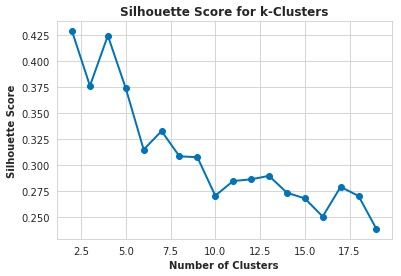
\includegraphics[width=8.5cm, height=6cm]{silhouette_scores.jpg}

Figure 2. Grouped boxplot of standardized cluster attributes.

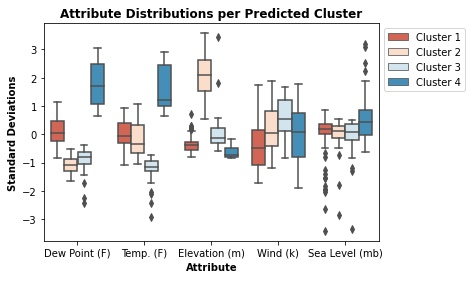
\includegraphics[width=8.5cm, height=6cm]{attribute_distribution.jpg}

Figure 3. Mapping of k-means predicted clusters to United States.

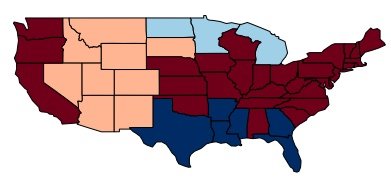
\includegraphics[width=8.5cm, height=6cm]{cluster_on_map.jpg}

\end{document}
